%
% include the class file for GMP 2018
%
\documentclass[submission]{gmp2018}

%%%%%%%%%%%%%%%%%%%%%%%%%%%%%%%%%%%%%%%%%%%%%%%%%%%%%%%%%%%%%%%%%%%%

\begin{document}

%
% put the title of your paper here
%
\title{Folding Cartons: }

%
% put your submission number here
% this number will appear instead of authors and affiliations if the class option "submission" is active
%
\SubNumber{{\color{red}{XXX}}}

%
% put the author names here
% use the second argument as a reference to the list of affiliations
% no authors and affiliations will appear if the class option "submission" is active
%
\author{Shuang Shan}{1}
\author{Yiting Ma}{1}
\author{Chengcheng Tang}{2}
\author{Xuejin Chen}{1}

%
% put the affiliations of the authors here
%
\affiliation{1}{University of Science and Technology of China}
\affiliation{2}{Stanford University}

%
% the rest is as usual
%

%%%%%%%%%%%%%%%%%%%%%%%%%%%%%%%%%%%%%%%%%%%%%%%%%%%%%%%%%%%%%%%%%%%%

\maketitle

\begin{abstract}
This paper provides an interactive system to construct three-dimensional carton model from two-dimensional design layouts, and simultaneously show these two views to asist users design box layouts more efficiently and productively. We also propose simple shape constrains related to edges and planes to implement the optimized construction along with the acquired information from interaction. To make the interaction simpler, we also provide sysmmetry detection and automatically detection of the vertices that need to be merged together, and allow users choose the right option.  
\end{abstract}

%%%%%%%%%%%%%%%%%%%%%%%%%%%%%%%%%%%%%%%%%%%%%%%%%%%%%%%%%%%%%%%%%%%%

\section{Introduction}
Cartons have been widely used in packaging industry to deliver various commodities including food items, daily necessities and electronic components. Instead of very basic packaging shapes like cubes, there exist multiple fantastic cartons to package wedding candies or take away coffee cups. These various designs increase much popularity, not to mention they're environmental friendly due to their recycling and degradability~\cite{Mullineux:2010:CSC:1739328.1739673}.

Cartons are usually designed based on experiance and trial-and-error, though recent years there are softwares developed to help designers improve efficiency and productivity, for example, KASEMAKE~\cite{KASEMAKE} can help users pick the existing structural designs and feed in required basic size and material, also users can re-import the finished artwork to show the print on the structural designs and fold it into a three-dimensinal view in seconds. There still comsumes much work and time to construct 3D model directly from 2D design layout. Moreover, it's sometimes intractable to fold an irregular box layout to final carton without instructions.

Researchers have studied papercraft problem for more than twenty years, they're primarily concerned with the following: (1) computational algorithm and mathmatic analysis for folding origami, as in~\cite{Ida:2007:MOC:1802954.1803021,Lang:1996:CAO:237218.237249,xl-idetc-14}; (2) problems on folding polygon and unfolding polyhedron~\cite{Bern:2003:UPC:636968.636970,O'Rourke:1998:FUC:646319.686376,Rourke2008Unfolding}, and some prooves to show the problem complexity of folding to polyhedron~\cite{Biedl:2005:NFP:1090462.1646553,Biedl2004When,Lubiw1996When}; (3) other specific structure folding problems, such as origami architectures~\cite{Le:2014:SCO:2574223.2574468,Li:2011:GSV:1964921.1964993,Li:2010:PAP:1833349.1778848,Ruiz:2013:GMP:2542355.2542360}, paper sliceforms~\cite{Le-Nguyen:2013:APS:2553684.2553686,McCrae:2011:SSB:2070781.2024202,Schwartzburg13}, Kinetogami which comprises multi-primitive and reconfigurable units folded from a single sheet of paper~\cite{Gao2013Kinetogami}; (4) applications to show the folding behaviour of paper~\cite{Thiel1998,Kishi:1998:OFP:786112.786279,Nimnual2007Virtual,Shimanuki2009Construction}. Although previous works sloved plenty problems in paper folding, they have not considered intelligent construction 3D models given 2D paper layouts. In this paper, we will focus on the carton folding problem and introduce shape optimization method to solve it.

In this paper, we try to construct 3D realization from 2D structural box design directly by shape optimization based on the information obtained from simple user interaction.  Besides, we allow users design the pattern in 2D layout, and visualize it in a 3D view, which can improve the efficiency a lot when designing a complicated texture. The contribution of this paper includes the following:

(1) We build an interactive system to design the 2D layout of cartons. It loads the specific type of layout and create the corresponding flat polymesh, by initialization and user interaction, we can finally construct the correct model of the carton.

(2) We propose simple shape constrains represented by a set of points to implement shape optimization. Observed from existing cartons, we can summarize edge constrain, coplane constrain and plane constrain to keep the shape of cartons. Besides, we also provide symmetry detection to give users suggestions. 

\section{Related Work}\label{sec:relatedwork}
\subsection{Reconsturction from single line drawings} 
Line drawings of three-dimensional objects have long been studied, and the main problem is still in reconstruction given projection on two-dimensional planes. Some researchers treat this task as optimization problem. \cite{Marill:1991:EHI:113057.113061} proposed MSDA(Minimize the Standard Deviation of Angles) principle to emulate the interpretion of line drawings as 3D objects. This new criterion is used by many other researchers later. \cite{Leclerc1992An} combined MSDA with the deviation from planarity as objective terms. \cite{Cao:2005:ORS:1097114.1097658} added symmetry measure of the objects to get more complicated results. Some other researchers try to solve this problem from the information theoretic point of view. \cite{Marill1992Why} minimized the description length of objects based on the idea that we usually pick the simplest one from infinite possibilities when we see the line drawing. \cite{Shoji20013} implemented the principle of minimizing the entropy of angle distribution between line segments using genetic algorithm. 

Different from the input above, ours are expanded structural layout of three-dimensional objects in 2D planes, the lackness of 3D topology is main cencern in our problem.

\subsection{Folding to polyhedron}

\cite{Lubiw1996When} provided an dynamic programming algorithm based on Aleksandrov's theorem to test whether a polygon can be folded into polyhedra which takes $O(n^2)$ time and space. \cite{O'Rourke:1998:FUC:646319.686376} examined three open problems on the subject of folding and unfolding. \cite{Biedl2004When} has studied in polynomial time to solve the question of when is the graph  orthogonally convex polyhedra given a graph, edge length and facial angles, also shown that it's NP-hard to decide whether the graph is orthogonally polyhedra or not. Rather than given graph, \cite{Biedl:2005:NFP:1090462.1646553} proved that if given a net along with the dihedral angle at each crease, we can know whether a net can be folded to a polyhedron in polynomial time, but it becomes NP-hard without the angles even adding constrains on orthogonal polyhedron, which results in more difficultes on more complex input.

Compared to our desired result, polyhedron is a set of polygons without overlap, nevertheless, our 3D model contains paste faces that needs to be fixed to another panel. These works above justify our problem being harder to solve causing by even intricater inputs.

\subsection{Paper craft} 
Various types of paper crafts have been studied in the field of computation and mathmatics. Origami is the Japanese traditional paper art of making different kind of objects by a single sheet of paper, and has been long studied since 1970s~\cite{KANADE1980279}. 

Lately, there have been newly researched automaticly generating a type of paper architecture named pop-ups. \cite{Li:2010:PAP:1833349.1778848} presented formulation of layouts, sufficient conditions to generate foldable and stable paper architectures, and proposed an automatic algorithm given any 3D models. Plenty papers studied this subject following the idea of Li's and make new improvements~\cite{Le:2014:SCO:2574223.2574468,Li:2011:GSV:1964921.1964993,Ruiz:2013:GMP:2542355.2542360}. Multiple types of papercraft have been researched as well, such as sliceforms~\cite{Le-Nguyen:2013:APS:2553684.2553686,McCrae:2011:SSB:2070781.2024202,Schwartzburg13}, which slots two sets of parallel paper patches together to make a foldable structure approximate to the given object. Cartons are also a kind of paper craft in another meaning.

\subsection{Carton Folding}
There are also some methods to solve the problem of carton folding. \cite{Song:2000:MPA:892954} modeled foldable objects as tree like multilink objects and use PRMs(probabilistic roadmap methods~\cite{Kavraki:1994:PRP:891758}) to find a sequence of motions to transform some configuration of a foldable object into another configuration. \cite{Mullineux:2010:CSC:1739328.1739673} provided a simulation of the carton during erection using a constraint-based approach. Both these work required the target state as a premise, while our work aim to generate the target configuration.

\subsection{Application on folding behaviour}
While researching on origami in the field of computational algorithm and geometric analysis, the simulation system is developed to visualize the folding behaviour of a single piece of paper. \cite{Thiel1998} provides a virtual origami system including the user interface to model folded paper and show animations of folding process. \cite{Kishi:1998:OFP:786112.786279} allows users create and edit the origami properties over the Web. \cite{Nimnual2007Virtual} presented an application for package folding practices in a virtual space.

Although these applications can model folded paper well, they need given parameters to construct the model, and we want to simplify these oprations by implementing shape optimization.

\subsection{Shape optimization}
Least square fitting is the common method to enforce shape constrains, and have been used successfully for interactive tools and physical simulation~\cite{Botsch:2006:PCP:1281957.1281959,Igarashi:2005:ASM:1186822.1073323}. \cite{Bouaziz:2012:SSD:2346796.2346802} unified a large varity of geometric constrain into one optimization framework, and provided simple, robust implementation. \cite{Tang:2014:FPM:2601097.2601213} solved constrained equations by Newton-type method in a fast way, and provided an interactive system to model meshed constrained by equalities and inequalities.In our paper, we implement the shape optimization by the method introduced in \cite{Bouaziz:2012:SSD:2346796.2346802} for its robustness and simplicity.

%%%%%%%%%%%%%%%%%%%%%%%%%%%%%%%%%%%%%%%%%%%%%%%%%%%%%%%%%%%%%%%%%%%%

\section{Overview}\label{sec:overview}
We aim to provide a system which help users design a accurate box structural layout and patterns on the surface by showing the three-dimensional view of the folded carton. We can expect a workflow like this: we import the specified type of input and show its 2D structural layout at the same time, then the system will give its initial 3D model and users can interact with the model by choosing the given suggestion to build the final carton model. After that, users can design the texture in 2D view and watch the 3D appearance immediately.

\begin{figure}
	\centering
	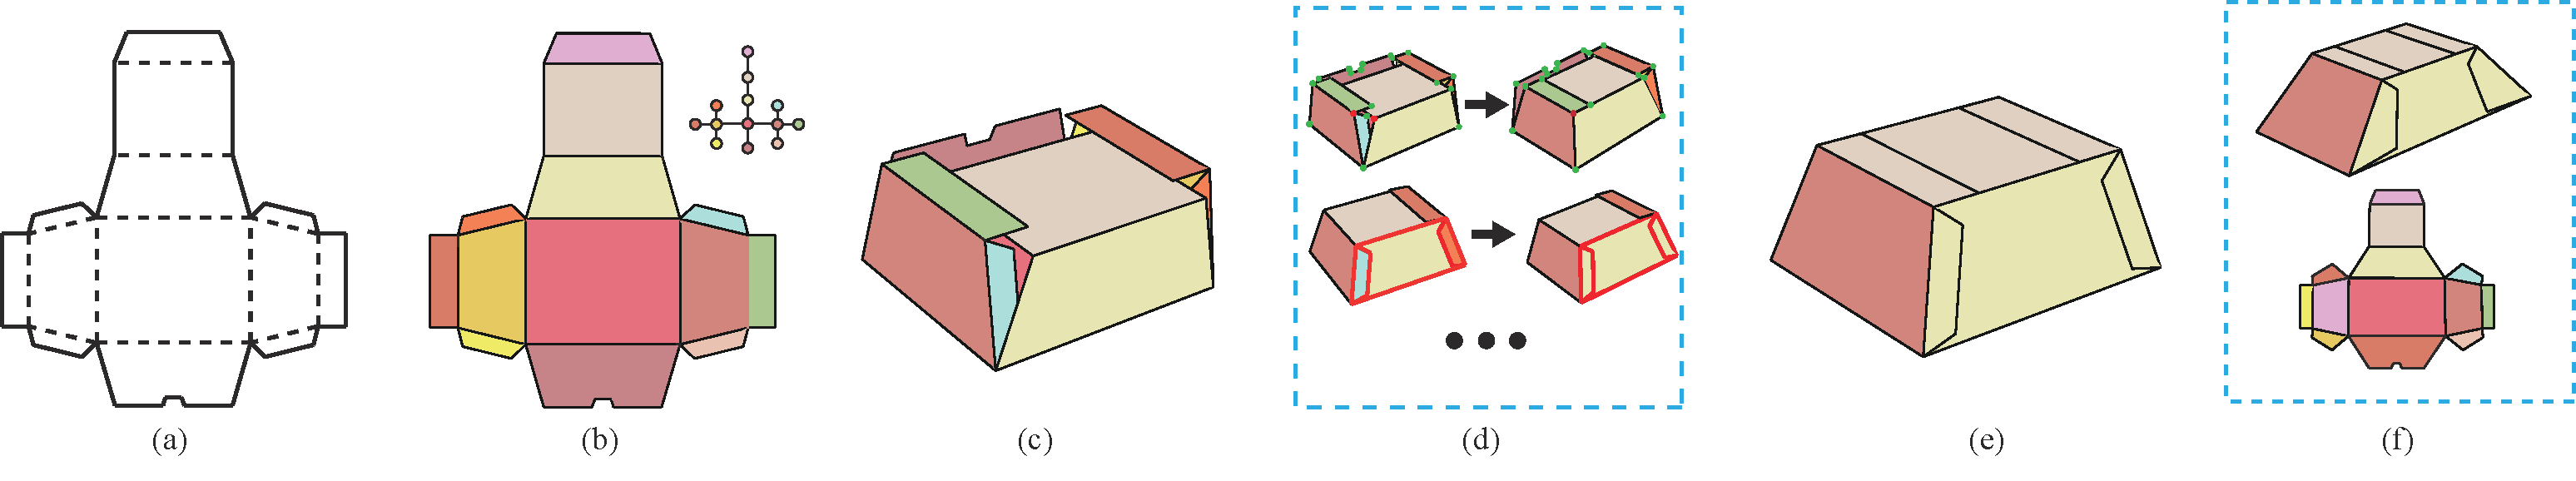
\includegraphics[width=0.9\textwidth]{images/overview.png}
	\caption{Given a 2D layout(a), we first create its 2D mesh(b), and by given a specific angle to each fold edge, we can construct the initial 3D model(c), the final model(d) is finally built through the optimization based on the information acquired from user interaction.}
	\label{fig:overview}
\end{figure} 

Figure~\ref{fig:overview} is our construction algorithm overview. Given a 2D layout Figure \ref{fig:overview}(a), we first create its 2D mesh Figure~\ref{fig:overview}(b), and by given a specific angle to each fold edge which will be explained later in section~\ref{sec:initialization} , we can construct the initial 3D model Figure~\ref{fig:overview}(c), the final model Figure~\ref{fig:overview}(d) is finally built through the optimization based on the information acquired from user interaction.

To formulate our problem, we assume that every plane is rigid which means the interior angle in each plane stays the same, but planes can be bent during folding. Furthermore, planes are connected by hinges at the boundry of the patches, and we assume that the planar layout has its front and back.

%%%%%%%%%%%%%%%%%%%%%%%%%%%%%%%%%%%%%%%%%%%%%%%%%%%%%%%%%%%%%%%%%%%%%

\section{Initialization}\label{sec:initialization}
In this section we explain the reason why we use a specific angle to each fold edge, and construct our initialized model. The basic idea is to interpret the folded state of a box as a series of rotation angles along each edge, where the problem of predicting folded state is turned into a problem of predicting these angles.

\subsection{Definitions and Notations}
As an input to our initialization, we expect a flat polymesh $L$ created from a 2D design layout of a box. As an output of our initialization, we deform the input polymesh into its 3D realization $R$ according to the predicted angles along each of its fold edges. A polymesh consists of a set of vertices, edges and faces $M = (V,E,F)$, the number of vertices, edges and faces vary from one mesh to another. However, a pair of $(L,R)$ as the the 2D layout and its corresponding 3D realization share the same topology and therefore they have the same number of vertices, edges and faces. A flat mesh as a 2D layout $L$ has its $z$ component of each vertex set to be a constant zero: $X_z(\mathbf{v}) \equiv 0$ where $X = (X_x,X_y,X_z)$ is the vertex coordinate, and its normal of each face set as $(0,0,1)^T$: $\mathbf{n}(f) \equiv (0,0,1)^T$, where $f \in F$.

\subsection{Objective Term}
Observe from our database includes 60 data pairs $(L,R)$, we summarize two common rules as our basic idea of initialization.

\noindent
\textbf{Plane perpendicularity} The adjacent planes should not be paralleled, and we encourage them to be perpendicular. The term used here is
\begin{equation}
\alpha_{pe} = \sum_{i = 1}^{n} [\sin^{-1}(\mathbf{n}_1 \cdot \mathbf{n}_2)]^{2},
\label{equ:perp}
\end{equation}
where $\hat{n}_1$ and $\hat{n}_2$ denotes all possible combinations of normals of adjacent planes, and $n$ is the number of such combinations.

\noindent
\textbf{Plane parallelism} It was observed that two planes with same shape are probably paralleled, so we encourage more planes with same shape to be paralleled. The term is
\begin{equation}
\alpha_{pa} = \sum_{i = 1}^{n} [\cos^{-1}(\mathbf{n}_1 \cdot \mathbf{n}_2)]^{2},
\label{equ:para}
\end{equation}
where $\hat{n}_1$ and $\hat{n}_2$ denotes all possible combinations of normals of disadjacent planes that have same shape,  and $n$ is the number of such combinations.

By implementing the CMA-ES(Covariance Matrix Adaptation Evolution Strategy)~\cite{CMAES} adding the above two constrains, we can have our initialization result shown in Figure~\ref{fig:initial}. Note that as our input variables are fold angles of edges, we use $cos\alpha$ to represent $\mathbf{n}_1 \cdot \mathbf{n}_2$ where $\alpha$ is the angle between these two normal vectors. 

We can see from the five examples shown in Figure~\ref{fig:initial}, the up three examples can have ideal results and the bottom two results are even not closed at last, which actually caused by the two constrains above lead to a result that each angle of each edge is always $\pi/2$. As a consequence, some irregular boxes will present a boxy shape which we will refine later by user interaction.

As for our initialization, we finially set $\pi/2$ to each angle and this causes more than half of boxes folded correctly in our database.

\begin{figure}
	\centering
	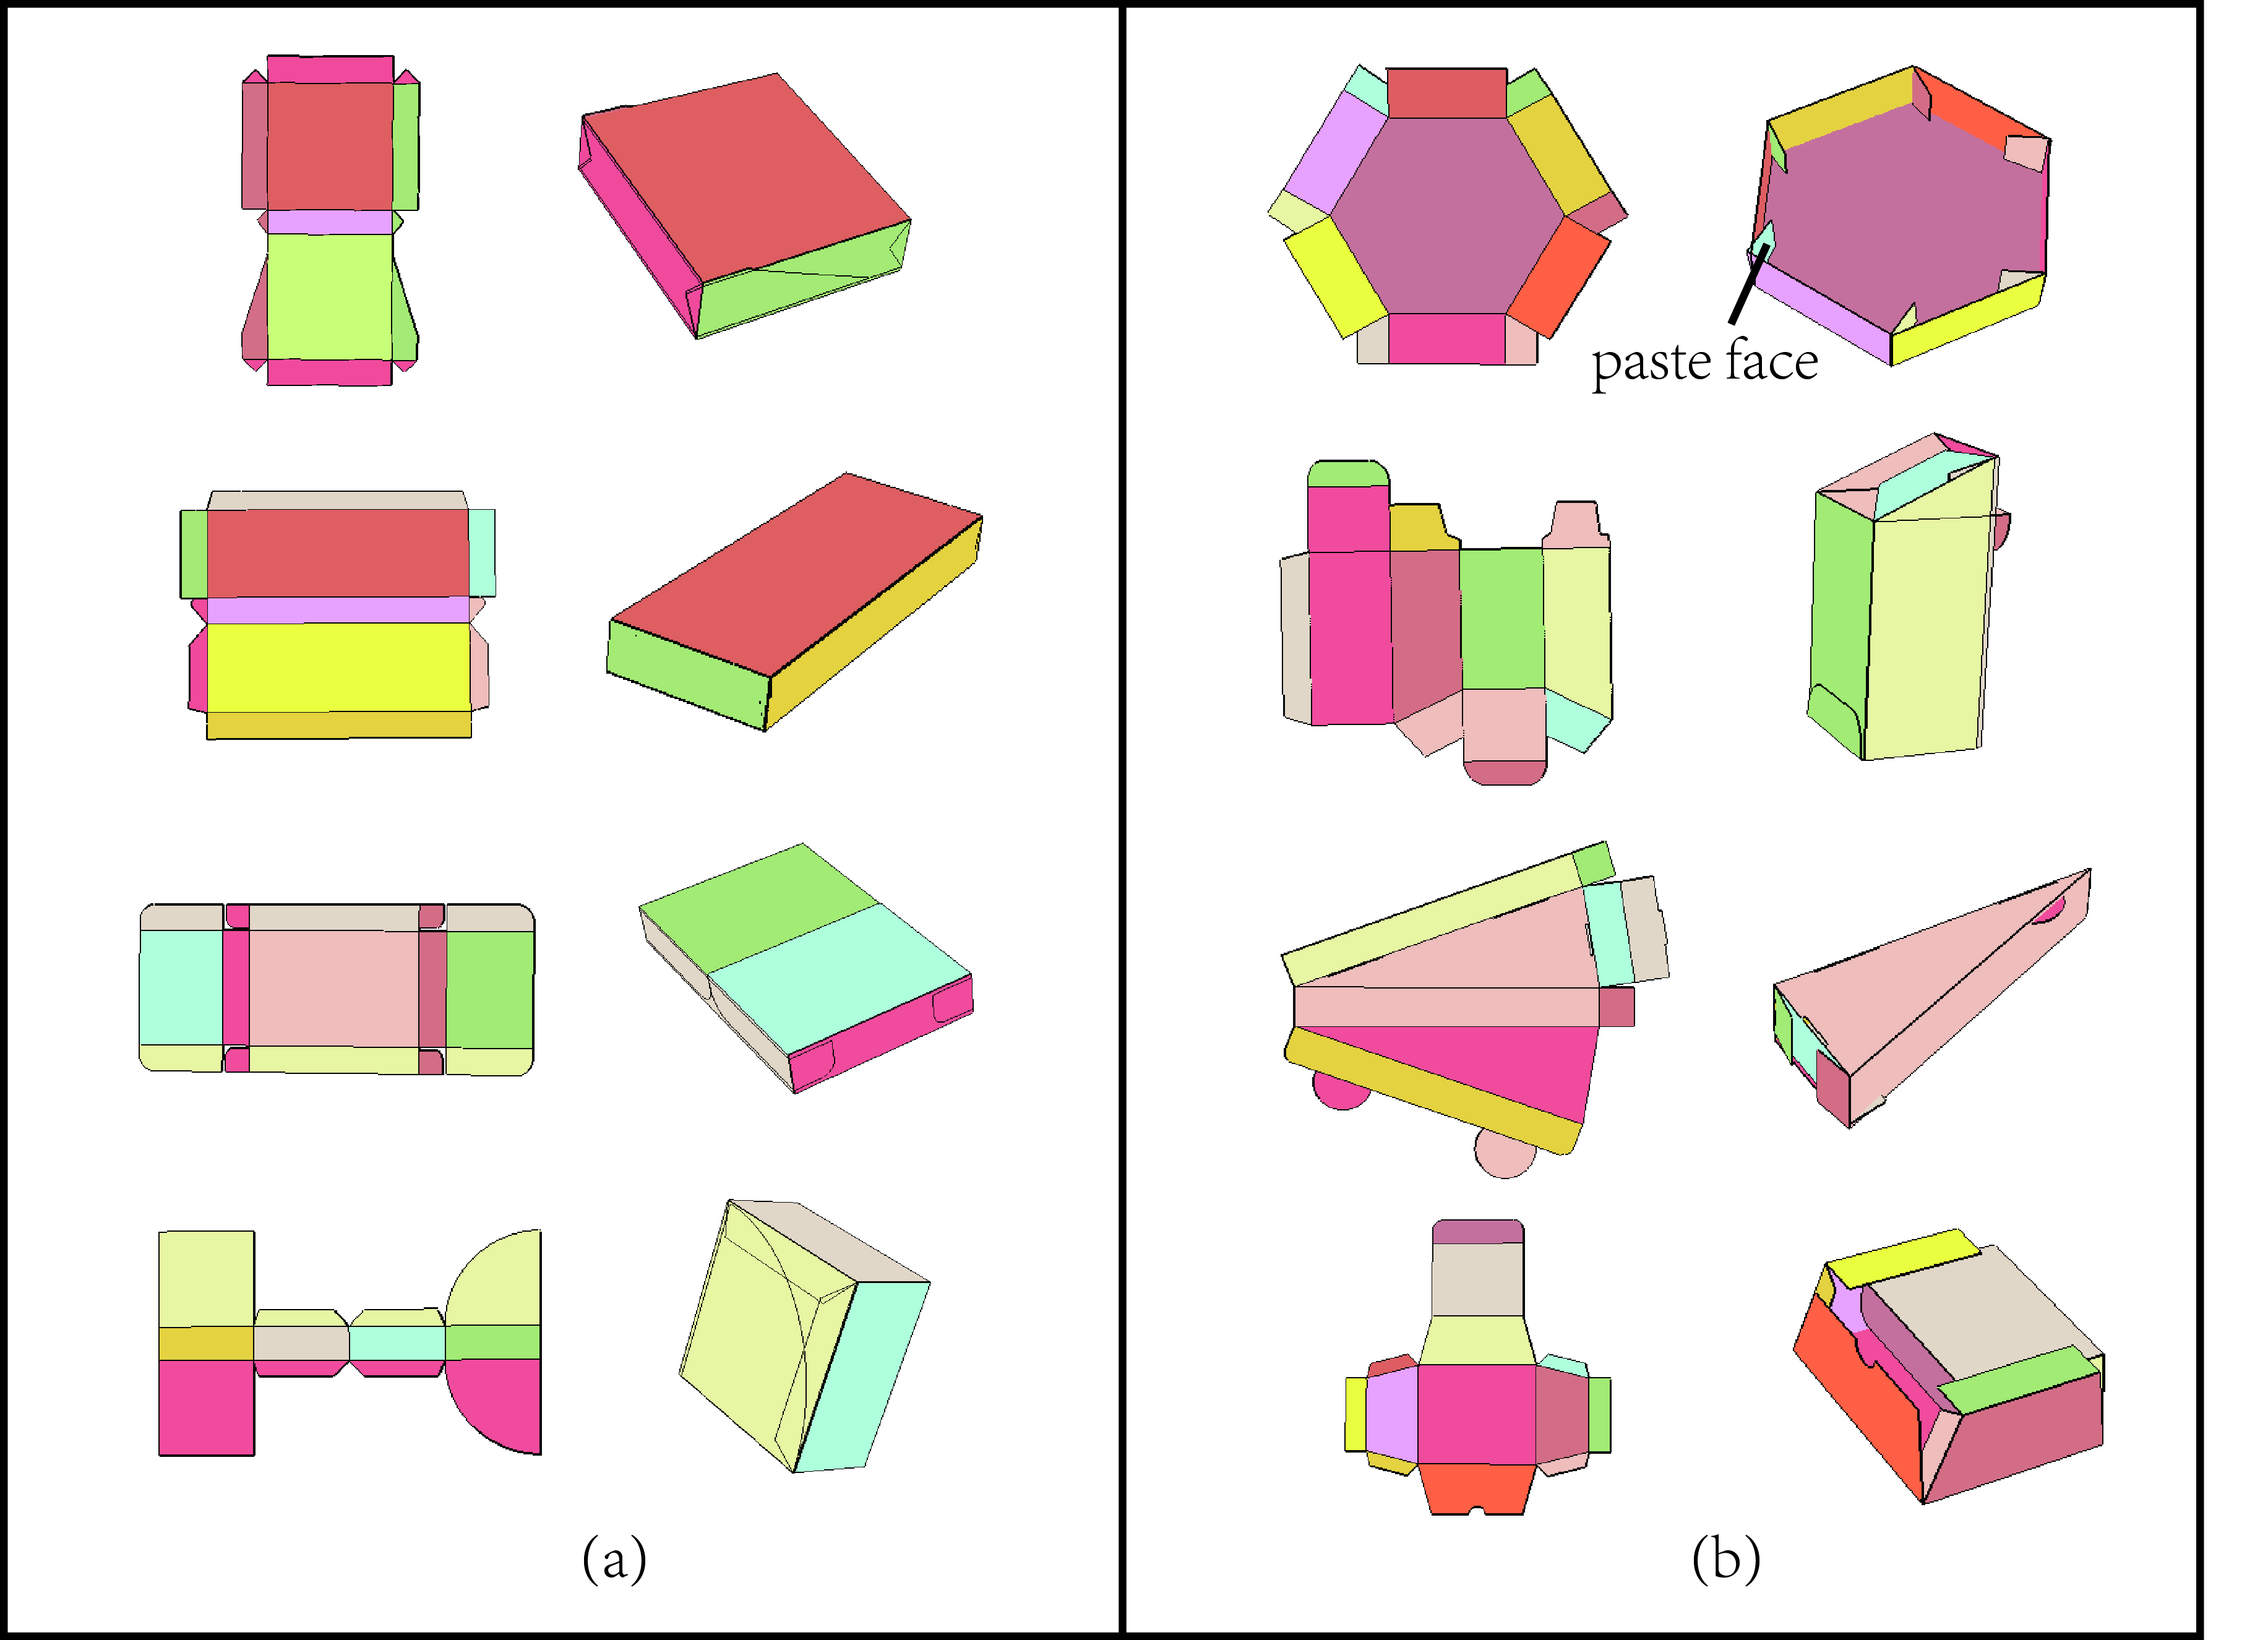
\includegraphics[width=0.9\textwidth]{images/initial.jpg}
	\caption{Initialized results of five examples. Each row is an example, and the first column is the 2D design layout, the second column is the polymesh created from layout, the third column is the initialized results optimized with the two constrains.}
	\label{fig:initial}
\end{figure}

%%%%%%%%%%%%%%%%%%%%%%%%%%%%%%%%%%%%%%%%%%%%%%%%%%%%%%%%%%%%%%%%%%%%%

\section{Shape Optimization}\label{sec:optimization}

After initialization, we still need to refine the results that have not folded into pleasing results. The main idea is to prescribe the shape constrains througn deforming using a set of vertices of the polymesh. Moreover, with the extra information acquired from user interaction, we can finally construct the ideal 3D realization compared to the ground truth. As you can notice, we choose the coordinate of vertices as our input instead of fold angles on edges, the reason is that constrains represented by vertices are more simple and intuitive than angles, and we can implement the algorithm introduced by  Bouaziz et al.~\cite{Bouaziz:2012:SSD:2346796.2346802} easily.

\subsection{Shape Constrain}\
We now introduce the constrains we mainly use in our construction method:

\noindent
\textbf{Edge Constrain} for each edge $\{e_j\}_{j=1...M}$, we have its start point $\mathbf{v}_{js}$ and end point $\mathbf{v}_{jt}$, then we have 
\begin{equation}
||\mathbf{v}_{js} - \mathbf{v}_{jt}||^2 = ||\mathbf{\hat{v}}_{js} - \mathbf{\hat{v}}_{jt}||^2,
\label{equ:edge}
\end{equation}
to ensure that the length of each edge stays the same.

\noindent
\textbf{Coplane Contrain} For each plane $\{p_k\}_{k=1 \dots P}$ and its normal $\mathbf{n}_k$, each line connected by two points $\mathbf{v}_{ka}, \mathbf{v}_{kb}$ on the plane is perpendicular to the normal.
\begin{equation}
\mathbf{n}_k \cdot (\mathbf{v}_{ka} - \mathbf{v}_{kb}) = 0.
\label{equ:coplane}
\end{equation}

\noindent
\textbf{Plane Constrain} For each plane $\{p_k\}_{k=1 \dots P}$, the length of each line connected by two non-adjacent points $\mathbf{v}_{ka}, \mathbf{v}_{kb}$ on the plane remains the same, so that the shape of each plane keeps unchanged.
\begin{equation}
||\mathbf{v}_{ka} - \mathbf{v}_{kb}||^2 = ||\hat{\mathbf{v}}_{ka} - \hat{\mathbf{v}}_{kb}||^2.
\label{equ:plane}
\end{equation}

The information acquired from user interaction will help us add enough constrains to solve the optimization problem, and one of the interaction is to choose the right given suggestion including points needed to be merged together. As for the point information, we can set the constrains like:

\noindent
\textbf{Point Constrain} 
\begin{equation}
\mathbf{v}_p - \mathbf{v}_q = 0,
\label{equ:point}
\end{equation}
if we need to move these two points $\mathbf{v}_p$, $\mathbf{v}_q$ into the same place.

When the above constrains still lead to an ill posed problem, a soft constrain will be introduced:

\noindent
\textbf{Irrelevant Point Constrain} Points $\{\mathbf{v}_i\}$ which are not in the same plane with $\mathbf{v}_p$ or $\mathbf{v}_q$, should be near the orignal location, and this constrain just take a light weight $w$, which is set 0.001 in our experiment. 
\begin{equation}
\mathbf{v}_i - \mathbf{\hat{v}}_i = 0.
\label{equ:irrelevant}
\end{equation}

{\color{red}{Figure~\ref{fig:constrain} visually shows the constrains above.}}

\begin{figure}
	\centering
	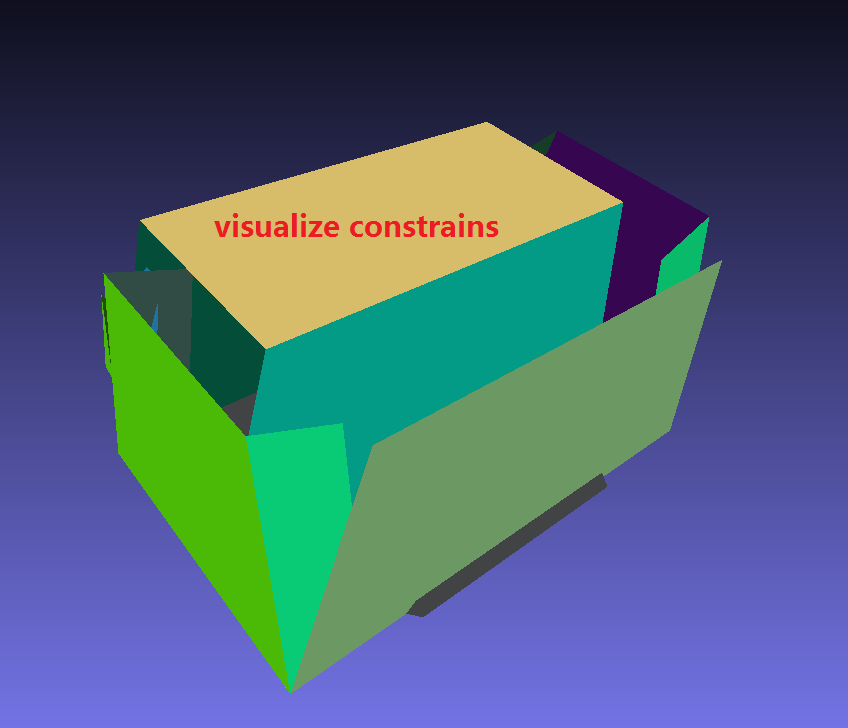
\includegraphics[width=0.9\textwidth]{images/constrains.png}
	\caption{}
	\label{fig:constrain}
\end{figure}


\subsection{Aided Detection}
In order to asist users construct the final carton interactively, we also provide symmetry detection and merging points detection.

\noindent
\textbf{merging points detection} Consider the initialization results can represent the ideal model partly, we detect the disadjacent vertices that have one edge with same length, and if their Euclidean distance is below a certain threshold, we regard these vertices as targets that need to be located in the same place.

\noindent
\textbf{symmetry detection} On account of the simplicity of the carton shape, we regard the vertices that have same length set of incident edges as symmetric pair.

%%%%%%%%%%%%%%%%%%%%%%%%%%%%%%%%%%%%%%%%%%%%%%%%%%%%%%%%%%%%%%%%%%%%%

\section{User Interaction}\label{sec:interaction}
After we initialize the flat mesh, we need to refine the model to final state through the shape constrain we propose and the information acquired from user interaction. We provide a set of operations to asist users construct the optimized model, such as selecting points that need to be merged together. Moreover, we can automatically detect the points that need to be located in one place and provide suggestions to allow users click the right option.

{\color{red}{Figure~\ref{fig:interface}} shows the interaction we mainly use in our system.}

\begin{figure}
	\centering
	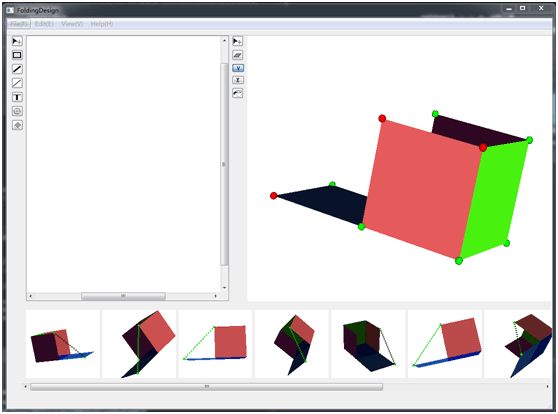
\includegraphics[width=0.9\textwidth]{images/ui.jpg}
	\caption{}
	\label{fig:interface}
\end{figure}

%%%%%%%%%%%%%%%%%%%%%%%%%%%%%%%%%%%%%%%%%%%%%%%%%%%%%%%%%%%%%%%%%%%%%

\section{Results and Discussion}\label{sec:result}
{\color{red}{show every step of results and analysis, show Figure~\ref{fig:result}, limitation, more results Figure~\ref{fig:more}}}


\begin{figure}
	\centering
	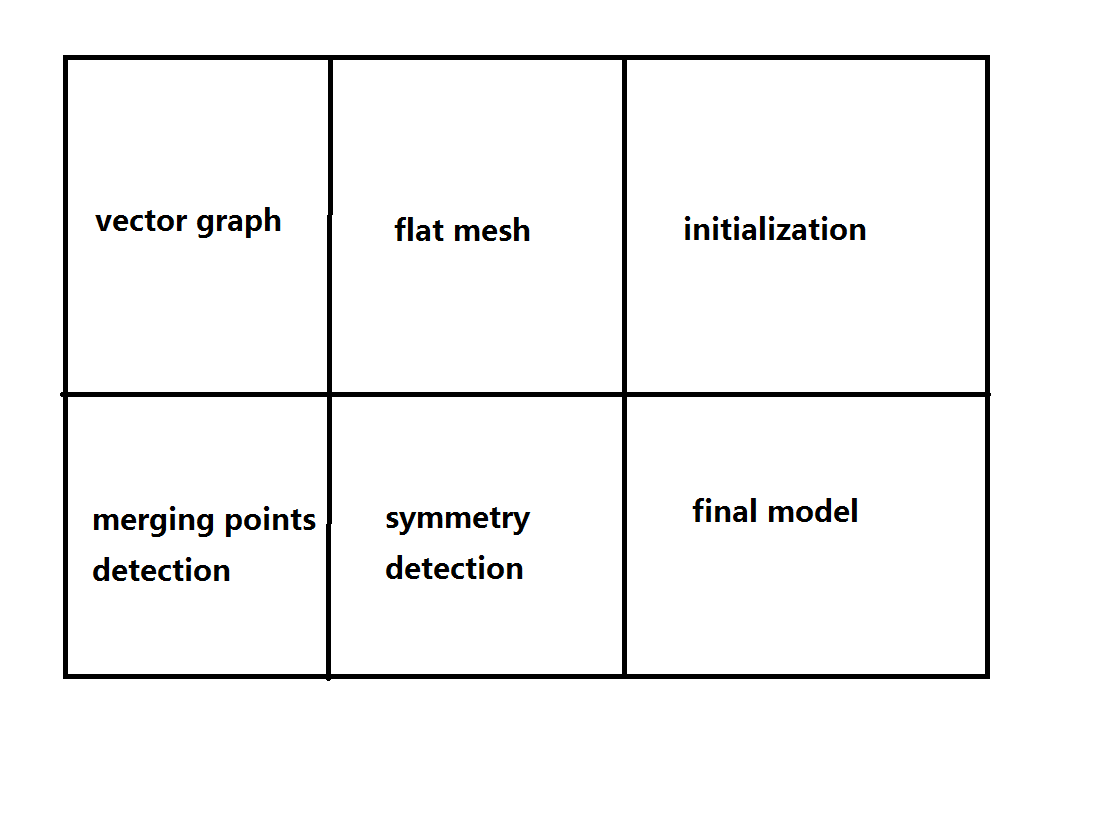
\includegraphics[width=0.9\textwidth]{images/result.png}
	\caption{}
	\label{fig:result}
\end{figure}

\begin{figure}
	\centering
	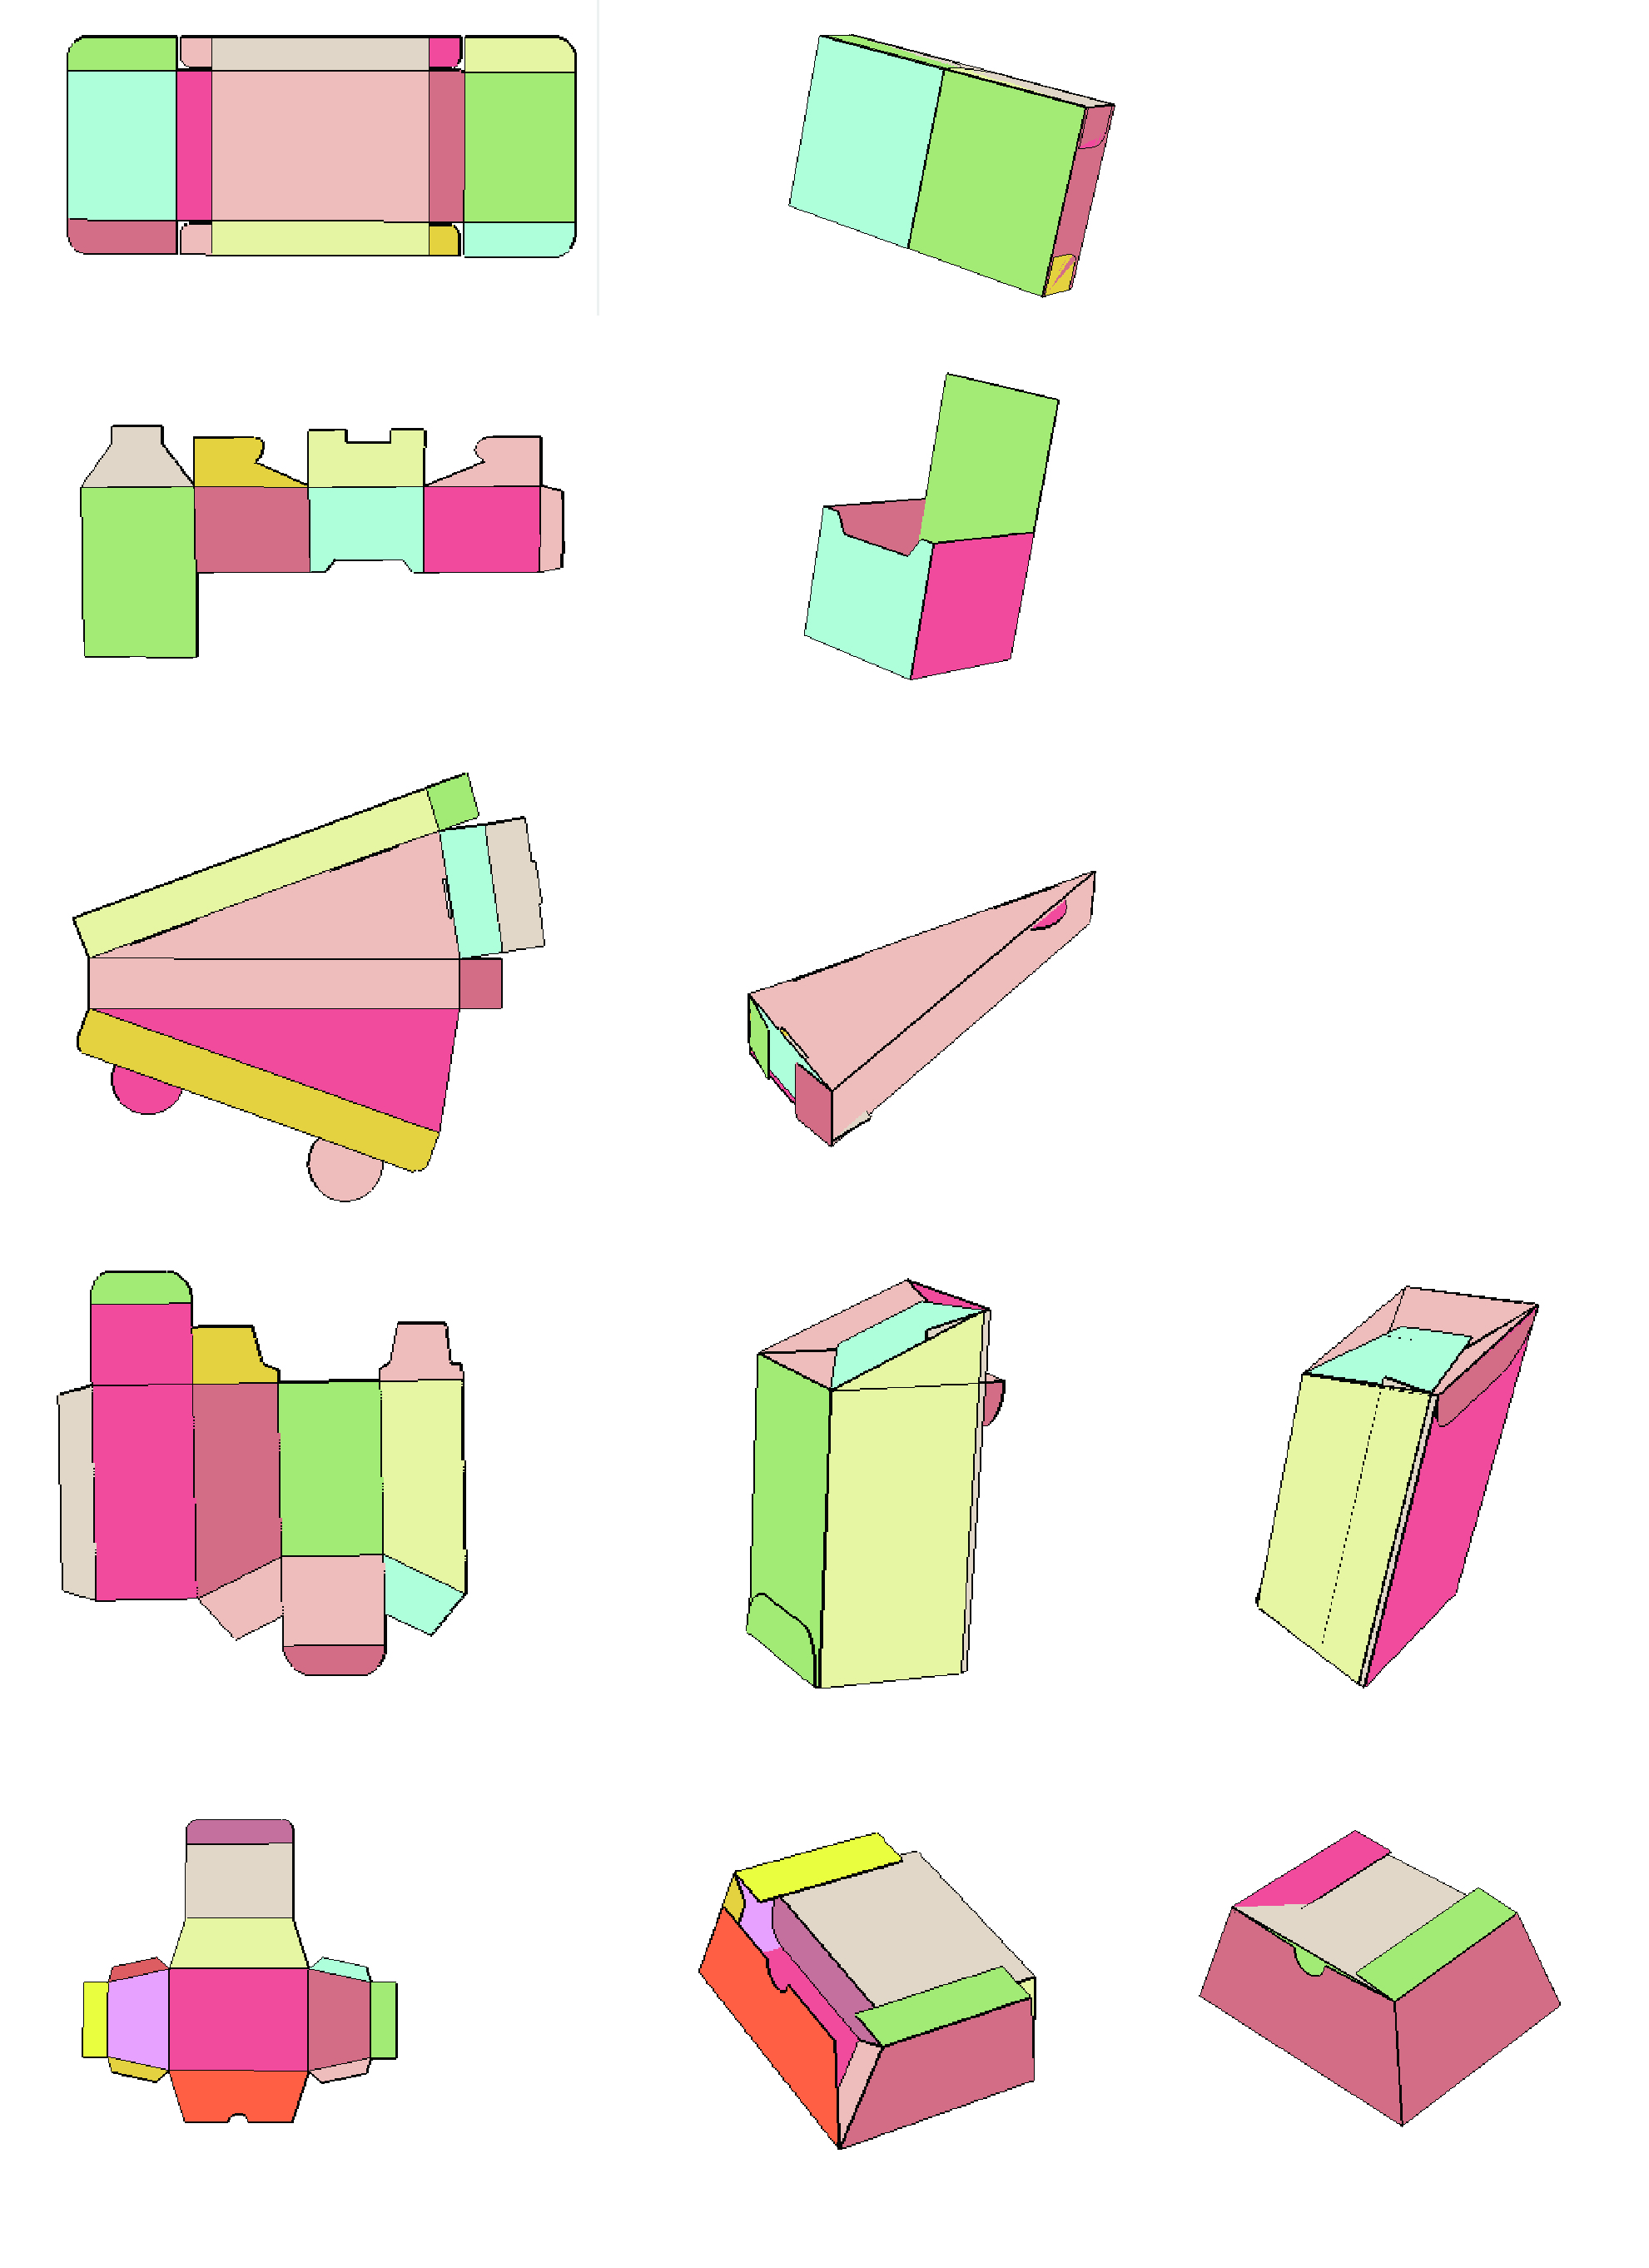
\includegraphics[width=0.9\textwidth]{images/more.png}
	\caption{}
	\label{fig:more}
\end{figure}

%%%%%%%%%%%%%%%%%%%%%%%%%%%%%%%%%%%%%%%%%%%%%%%%%%%%%%%%%%%%%%%%%%%%%

\section{Conclusion and Future Work}\label{sec:conclusion}
In this paper, we present an interactive modeling system to construct 3D carton realization from 2D expanded structural layout. We also provide simple shape constrains of cartons to implement optimization on the initial 3D models, which can asist users generate the ideal model efficiently and productively. The direction of future work is adding more operations to our system, includes automatically refining the 2D layouts by 3D models, adding the paste face through stablity detection. 

%%%%%%%%%%%%%%%%%%%%%%%%%%%%%%%%%%%%%%%%%%%%%%%%%%%%%%%%%%%%%%%%%%%%%

%\begin{theorem}\label{theorem:pi}
%Aliquam nec sapien sit amet diam molestie tristique vitae sit amet libero,
%\begin{equation}\label{eq:pi}
%\pi = \sqrt{12}\sum^\infty_{k=0} \frac{(-3)^{-k}}{2k+1}.
%\end{equation}
%\end{theorem}

%\begin{proof}
%Curabitur metus lorem, rhoncus nec ullamcorper quis, varius eget neque. Phasellus et turpis quis massa porta tincidunt. Donec fringilla luctus libero, at adipiscing justo ullamcorper non. Mauris magna ipsum, semper eget hendrerit nec, ornare sit amet neque. Nullam elementum arcu eget tellus porta mattis.
%\end{proof}

%\noindent
%Morbi ut lorem lectus. Etiam quis dolor justo, according to~\eqref{eq:pi}. Duis suscipit laoreet sollicitudin. Phasellus lacinia adipiscing tortor at posuere. Integer eget neque ac lacus vestibulum sollicitudin. Mauris vitae lacus dui. Aenean ultrices iaculis faucibus. Suspendisse congue, lectus in vulputate convallis, magna eros gravida mi, a molestie metus urna a nibh. Suspendisse adipiscing gravida ullamcorper.
%


%\begin{corollary}
%Etiam quis mauris orci. Nam blandit elementum diam a molestie. Suspendisse ultricies auctor urna, quis sagittis metus semper vel. Cras vel nisi felis.
%\end{corollary}

%%%%%%%%%%%%%%%%%%%%%%%%%%%%%%%%%%%%%%%%%%%%%%%%%%%%%%%%%%%%%%%%%%%%

\bibliographystyle{abbrv}
\bibliography{ref}

\end{document}
